\documentclass[12pt,a4paper]{article}
\usepackage[utf8]{inputenc}
\usepackage{graphicx}
\usepackage{amsmath}
\usepackage{amssymb}
\usepackage{geometry}
\geometry{margin=1in}
\usepackage{float}
\usepackage{tabularx}
\usepackage{setspace}
\onehalfspacing
\setcounter{tocdepth}{4}
\usepackage{titlesec}
\titleformat{\paragraph}[block]{\normalfont\normalsize\bfseries}{\theparagraph}{1em}{}
\titlespacing*{\paragraph}{0pt}{*1}{*0.5}
\usepackage[colorlinks=true, linkcolor=black, urlcolor=blue, citecolor=blue]{hyperref}
\usepackage{tikz}
\usepackage{pgfplots}
\pgfplotsset{compat=1.18}

\title{Problems}
\author{Mert Samet Kayacıoğlu}
\date{\today}
\newpage

\begin{document}

\maketitle
\thispagestyle{empty}
\newpage
\tableofcontents
\newpage

\begin{center}
\Large \textbf{Problems}
\end{center}

\section{Algebra}

\subsection{Equations}

\subsubsection{Irrational Equations}

\paragraph{Problem 1 - Nested Radicals}

Solve the equation.

\noindent\textbf{Source:} \href{https://www.youtube.com/watch?v=sdPtTqu3c0A}{Fun Algebra Problem!}

\[
\sqrt{1 + \sqrt{1 + x}} = \sqrt[3]{x}
\]

\subparagraph{Solution}
\[
(1 + \sqrt{1 + x})^{\frac12} = x^{\frac13}
\]
\[
1 + \sqrt{1 + x} = x^{\frac23}
\]
\[
1 + x = \left( x^{\frac23} - 1 \right)^2
\]
\[
1 + x = x^{\frac43} - 2x^{\frac23} + 1
\]
\[
x = x^{\frac43} - 2x^{\frac23}
\]
\[
x \left( 1 - x^{\frac13} \right) = -2x^{\frac23}
\]
\[
1 - x^{\frac13} = -2x^{-\frac13}
\]
\[
2x^{-\frac13} + 1 - x^{\frac13} = 0
\]
\[
t = x^{\frac13} \quad (t \in \mathbb{R}), \  \ 2t^{-1} + 1 - t = 0
\]
\[
\Rightarrow\ 2 + t - t^{2} = 0 \quad\Longleftrightarrow\quad t^{2} - t - 2 = 0
\]
\[
(t-2)(t+1)=0 \ \Rightarrow\ t=2 \ \text{ or } \ t=-1
\]
\[
\text{Since } \sqrt{1+\sqrt{1+x}}\ge 0 \Rightarrow x^{\frac13}\ge 0 \Rightarrow t\ge 0
\]
\[
\therefore\ t=2 \quad\Rightarrow\quad\boxed{x=t^{3}=8}
\]
\noindent\textbf{Verification:}
\[
\sqrt{1+\sqrt{1+8}}=\sqrt{1+3}=2=\sqrt[3]{8}
\]
\[
x=8
\]

\newpage
\paragraph{Problem 2 - Infinite Nested Radicals}

Solve the equation.

\noindent\textbf{Source:} \href{https://www.youtube.com/watch?v=iOtjKo1Xsg0}{Solving for Infinite x's!}

\[
5=\sqrt{x+\sqrt{\,2x+\sqrt{\,x+\sqrt{\,2x+\sqrt{\,x+\sqrt{\,2x+\cdots}}}}}}
\]

\subparagraph{Solution}
\[    
    s = \sqrt{2x + \sqrt{x + \sqrt{2x + \cdots}}}
\]
\[    
    s=\sqrt{2x+\underbrace{\sqrt{x+s}}_{=\,5}}=\sqrt{2x+5}
\]
\[
5=\sqrt{x+s}\;\Longrightarrow\; s=25-x
\]
\[
25 - x = \sqrt{2x + 5}
\]
\[
(25-x)^2=2x+5 \;\Longrightarrow\; x^2-52x+620=0
\]
\[
\Delta = b^2 - 4ac = (-52)^2 - 4 \cdot 1 \cdot 620
= 2704 - 2480 = 224
\]
\[
x = \frac{-b \pm \sqrt{\Delta}}{2a}
= \frac{-(-52) \pm \sqrt{224}}{2}
= \frac{52 \pm 4\sqrt{14}}{2}
= 26 \pm 2\sqrt{14}.
\]
\[
s = 25 - x \ge 0 \;\Rightarrow\; x \le 25
\]
\[
\boxed{x = 26 - 2\sqrt{14}}
\]
\noindent\textbf{Verification:}
\[
\sqrt{x} \approx 4.30310\ldots
\]
\[
\sqrt{x + \sqrt{2x}} \approx 4.96005\ldots
\]
\[
\sqrt{x + \sqrt{2x + \sqrt{x}}} \approx 4.99460\ldots
\]
\[
\sqrt{x + \sqrt{2x + \sqrt{x + \sqrt{2x}}}} \approx 4.99969\ldots
\]
\[
\sqrt{x + \sqrt{2x + \sqrt{x + \sqrt{2x + \sqrt{x}}}}} \approx 4.99995
\]
\[
\sqrt{x + \sqrt{2x + \sqrt{x + \sqrt{2x + \sqrt{x + \sqrt{2x}}}}}} \approx 4.99999\ldots
\]

\newpage
\subsubsection{Absolute Value Equations}

\paragraph{Problem 3 - Quadratic Absolute Value Equation}

Solve the equation graphically and algebraically.

\noindent\textbf{Source:} Galatasaray University, Math I Midterm Exam 2022-2023, Damien Berthet

\[
    2|x - 1| = x^{2} - 2
\]

\subparagraph{Solution\linebreak}

\textbf{Graphic method :}

\begin{center}
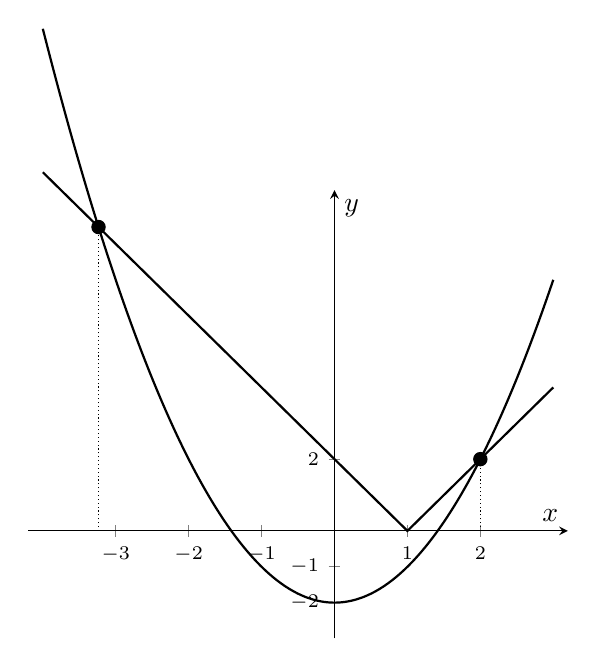
\begin{tikzpicture}
  \pgfmathsetmacro{\xleft}{-1 - sqrt(5)} 
  \pgfmathsetmacro{\xright}{2}
  \pgfmathsetmacro{\yleft}{\xleft*\xleft - 2}
  \pgfmathsetmacro{\yright}{\xright*\xright - 2}

  \begin{axis}[
    axis lines=middle,
    xmin=-4.2, xmax=3.2,
    ymin=-3,   ymax=9.5,
    xlabel={$x$}, ylabel={$y$},
    xtick={-3,-2,-1,0,1,2},
    ytick={-2,-1,0,2},
    ticklabel style={font=\scriptsize},
    clip=false
  ]

\addplot[domain=-4:3, samples=400, thick]
{x^2 - 2};

\addplot[domain=-4:3, samples=400, thick]
{2*abs(x-1)};

\addplot[only marks, mark=*, mark size=2.4pt]
coordinates {(\xleft,\yleft) (\xright,\yright)};

\draw[densely dotted] (axis cs:\xright,0) -- (axis cs:\xright,\yright);
\draw[densely dotted] (axis cs:\xleft,0)  -- (axis cs:\xleft,\yleft); 

\end{axis}
\end{tikzpicture}
\end{center}

\[
    S = \{2, x_1\} \quad \text{avec} \quad x_1 < -3.
\]

\textbf{Calculation :}
\[
    2|x - 1| = x^{2} - 2
    \iff
    \begin{cases}
        2x - 2 = x^{2} - 2 \\[2pt]
        x > 1
    \end{cases}
    \ \text{or}\
    \quad\begin{cases}
        -2x + 2 = x^{2} - 2 \\[2pt]
        x < 1
    \end{cases}
\]
\[
    \iff x = 2 \ \text{or}\
    \begin{cases}
        x^{2} + 2x - 4 = 0 \\[2pt]
        x < 1
    \end{cases}
 \]
\[   
    \iff x=2 \ \text{or}\
    \begin{cases}
        x = -1 \pm \sqrt{5} \\[2pt]
        x < 1
    \end{cases}
\]
\[
    \boxed{S = \{ 2,\, -1 - \sqrt{5} \}}
\]

\end{document}